%
%
%
%
%
%
%
%
%
%
%
%
%
%
%
%
%
%
%
%
%
%
%
%
%
%
%
%
\begin{document}

\title{Fast Inexact Graph Matching \\ with Applications in Statistical Connectomics}
% \title{A Quadratic Assignment Problem Approach to Graph Matching: Applications in Statistical Connectomics}

\author{Joshua T.~Vogelstein, John M.~Conroy, Louis J.~Podrazik, Steven G.~Kratzer, 
        Donniell E.~Fishkind, 
		R.~Jacob~Vogelstein,
        and~Carey~E.~Priebe% <-this % stops a space
\IEEEcompsocitemizethanks{\IEEEcompsocthanksitem J.T. Vogelstein, D.E. Fishkind, and C.E. Priebe are with the Department
of Applied Mathematics and Statistics, Johns Hopkins University, Baltimore, MD 21218. 
%\protect\\
% note need leading \protect in front of \\ to get a newline within \thanks as
% \\ is fragile and will error, could use \hfil\break instead.
E-mail: \{joshuav,def,cep\}@jhu.edu, \{conroyjohnm,ljpodra,sgkratz\}@gmail.com, jacob.vogelstein@jhuapl.edu
\IEEEcompsocthanksitem J.M. Conroy, L.J. Podrazik and S.G. Kratzer are with Institute for Defense Analyses, Center for Computing Sciences, Bowie, MD 20708.
\IEEEcompsocthanksitem R.J. Vogelstein is with the Johns Hopkins University Applied Physics Laboratory, Laurel, MD, 20723.}% <-this % stops a space
\thanks{This work was partially supported by the Research Program in Applied Neuroscience.}}
 
% The paper headers
\markboth{IN PREP}%
{Graph Classification}

\IEEEcompsoctitleabstractindextext{%
\begin{abstract}
It is becoming increasingly popular to represent myriad and diverse data sets as graphs.  When the labels of vertices of these graphs are unavailable, graph matching (GM)---the process of determining which permutation assigns vertices of one graph to those of another, maintaining the adjacency structure---is a computationally daunting problem.  This work presents an inexact strategy for GM.  Specifically, we relax the feasible region to its convex hull and then apply a well known and efficient nonlinear programming algorithm, Frank-Wolfe, to the objective function.  Though this relaxation is convex, the point around which the local approximation is made determines the optimum.  We therefore consider a number of initializations based on the geometry of the convex hull.  Multiple restarts of this algorithm lead to performance that exceeds the previous state-of-the-art in \emph{all} of 16 benchmark tests.  Moreover, this approach is fast, scaling cubically with the number of vertices, requiring only a few minutes on standard modern laptops for graphs with up to a few hundred vertices.  We illustrate this approach via a brain-graph (``connectome'') application in which vertices represent neurons in a small nematode brain (the \emph{Caenorhabditis elegans} worm), and edges represent either chemical or electrical synapses.  For every chemical connectome and several electrical connectomes, this approach found the optimal solution.  Although this strategy already natively operates on  unweighted and weighted graphs, either directed or undirected, we propose a number of possible extensions, and make all code available.
\end{abstract}

% Note that keywords are not normally used for peer review papers.
\begin{keywords}
statistical inference, graph theory, network theory, structural pattern recognition, connectome.
\end{keywords}}


% make the title area
\maketitle
\IEEEdisplaynotcompsoctitleabstractindextext
\IEEEpeerreviewmaketitle



\section{Introduction}

% define a graph labeling function as any algorithm that assigns a label to each vertex of a graph: $Q_n: \mc{A}, \Xi^n \mapsto \mc{L}$, where $\Xi \subseteq \mc{G}$, for example, $\Xi=\mc{A}$ (note that we have actually defined a sequence of graph labeling functions).  Remember that we have defined $\mc{L}$ as a subset of $[n_v]$, so each vertex need not have a unique label.  

\IEEEPARstart{A}{} graph matching (GM) algorithm is any algorithm whose goal is to ``align'' any pair of graphs such that each vertex in one graph can be ``assigned'' to its corresponding vertex in the other graph.  Perhaps due to its complex computational properties (it is $\mc{NP}$-hard \cite{Garey1979}), GM has received widespread attention in both the mathematical graph theory and computer science communities \cite{Conte2004}.  Moreover, the potential span of applications of graph matching algorithms is vast, ranging from neural coding \cite{Richiardi2010} to machine vision \cite{Wiskott1997}.  

Our motivation for this work includes the bourgeoning field called ``connectomics'': the study of brain-graphs.  In brain-graphs,  vertices represent (collections of) neurons and edges represent either functional dependencies or structural connections \cite{Sporns2010}.  In some scenarios, vertices are labeled.  For example, when vertices represent single neurons in invertebrates \cite{WhiteBrenner86} or macro-anatomical gyral regions in vertebrates \cite{Biswal2010,Bullmore2010}.  However, in other scenarios, even whether vertices can be labeled is questionable.  For example, if one desired to compare brain-(sub)graphs from parts of brains across species or within vertebrate organisms, there is no known vertex assignment.  In these scenarios GM might be an important element of any statistical analysis of these brain-graphs \cite{VP11_sigsub, VP11_unlabeled}.


We therefore propose a novel inexact graph matching algorithm.  The intuition is relatively simple: GM is computationally difficult because the underlying feasible region is non-differentiable and the implied objective function is multimodal.  A common approach to approximating difficult nonlinear programming problems is to relax the constraints on the feasible region.  By relaxing the non-differentiable constraint, any gradient based algorithm may be applied to the problem \cite{Mangasarian1987}. Unfortunately, the multimodality of the solution space implies that the initialization will, in general, be important.  Multiple ``principled'' restarts can potentially facilitate an efficient stochastic search strategy.  

This manuscript describes an algorithm that approximately solves a relaxed version of graph matching in cubic time (with very small leading constants).  Via numerical experiments, we demonstrate that this approach outperforms several state-of-the-art algorithms on all tests in a standard benchmark library \cite{Burkard1997}, indicating both its efficiency and its effectivity. We then test this approach on a brain-graph matching problem: matching the brain-graphs of a small nematode with $302$ vertices.  We are able to find the optimal solution after $3$ restarts for each randomly permuted example.  We are therefore optimistic that this algorithm will be useful for the massive graphs ($\mc{O}(10^5)$ vertices)  promised to arise due to various ongoing connectome projects \cite{HCP,OCP}.










\section{Methods} % (fold)
\label{sec:methods}


\subsection{Preliminaries} % (fold)
\label{sub:preliminaries}

% subsection preliminaries (end)

A labeled graph $G=(\mc{V},\mc{E})$ consists of a vertex set s $\mc{V}$, where $|\mc{V}|=n$ is number of vertices and an edge set $\mc{E}$, where $|\mc{E}| \leq n^2$. Note that we are not restricting our formulation to be directed or exclude self-loops. Given a pair of graphs, $G_1=(\mc{V}_1,\mc{E}_1)$ and $G_2=(\mc{V}_1,\mc{E}_1)$, where $|\mc{V}_1|=|\mc{V}_2|=n$, 
let $\pi: \mc{V}_1 \to \mc{V}_2$ be a permutation function (bijection), and consider the following two closely related problems:
% A pair of graphs, $G_1$ and $G_2$, are isomorphic if and only if the following \emph{isomorphism criterion} holds: there exists a $\pi \in \Pi$ such that . 
% Let $A$ be the adjacency matrix representation of graph such that $A_{uv}=1$ if there is an edge from $u$ to $v$, and $A_{uv}=0$ otherwise. 
% Note that the below follows for directed/undirected and loopy/non-loopy graphs.
% $u \sim v \in \mc{E}$ and $A_{uv}=0$ otherwise.  
% Let  $\Pi$ be the set of permutation functions, where a permutation function (bijection) $\pi: \mc{V} \to \mc{V}$ (re-)orders the elements of the set $\mc{V}$.  Given a pair of $n \times n$ adjacency matrices, $A=(a_{uv})$ and $B=(b_{uv})$, consider the following two problems:
\begin{itemize}
	\item \textbf{Graph Isomorphism (GI):}  Does there exist a $\pi \in \Pi$ such that $(u,v) \in \mc{E}_1$ if and only if $(\pi(u),\pi(v)) \in \mc{E}_2$. 
		\item \textbf{Graph Matching (GM):} Which $\pi$ (if any) satisfies the above isomorphism criterion?
\end{itemize}

% \begin{itemize}
% 	% $\PmcP$ (if any) satisfies $QAQ\T=B$?
% 	\item \textbf{Linear Assignment Problem (LAP):} 
% 	\begin{align}
% 		\text{minimize}_{\pi \in \Pi} \sum_{u \in \mc{V}} a_{u \pi(v)}
% 	\end{align}
% 	\item \textbf{Quadratic Assignment Problem (QAP):} 
% 	\begin{align}
% 		\text{minimize}_{\pi \in \Pi} \sum_{u,v \in \mc{V}} a_{\pi(u) \pi(v)}b_{uv}
% 	\end{align}
% \end{itemize}

Both GI and GM are computationally difficult. GM is clearly harder than GI, since solving GM also solves GI, but not vice versa. It is not known whether GI is in complexity class $\mc{P}$ \cite{Fortin1996}.  In fact, GI is one of the few problems for which, if $\mc{P} \neq \mc{NP}$, then GI might reside in an intermediate complexity class called $\mc{GI}$-complete.  GM, however, is known to be in $\mc{NP}$-complete.    
 % There exist no known algorithms for which worst case behavior is polynomial \cite{Fortin1996}.  While GM is known to be $\mc{NP}$-hard, it remains unclear whether GI is in $\mc{P}$, $\mc{NP}$, or its own intermediate complexity class, $\mc{NP}$-isomorphism (or isomorphism-complete).  
Yet, for large classes of GI and GM problems, linear or polynomial time algorithms are available \cite{Babai1980}.  Moreover, at worst, it is clear that GI is only ``moderately exponential,'' for example, $\mc{O}(\exp\{n^{1/2 + o(1)}\})$ \cite{Babai1981}.  Unfortunately, even when linear or polynomial time GI or GM algorithms are available for special cases of graphs, the constants are typically unbearably large.  For example, if all graphs have degree less than $k$, there is a linear time algorithm for GI.  However, the hidden constant in this algorithm is $512k^3!$ \cite{Chen1994}.  

Because we are interested in solving GM for graphs with $\mc{O}(10^6)$ or more vertices, exact GM solutions will be computationally intractable. As such, we develop a fast inexact graph matching algorithm.   Our approach is based on formulating GM as a quadratic assignment problem.  Below, we introduce assignment problems, and reiterate their close relationship to GI and GM \cite{Burkard2009}.

% We therefore determined the average complexity of our algorithm \emph{and} the leading constants.  Figure \ref{fig:scaling} suggests that our algorithm is not just cubic in time, but also has very small leading constants ($\approx 10^{-7}$ seconds), making using this algorithm feasible for even reasonably large graphs.


\subsection{Assignment Problems} % (fold)
\label{sub:assignment_problems}

Both GI and GM can be cast as assignment problems.  Let $A=(a_{uv})$ and $B=(b_{uv})$ correspond to the adjacency matrix representations of graphs $G_1$ and $G_2$, respectively.  That is, $a_{uv}=1$ if and only if $(u,v) \in \mc{E}_1$, and zero otherwise (and similarly for $B$ and $G_2$). Now, GI may be stated thusly:  does there exist a $\pi \in \Pi$ such that $a_{uv}=b_{\pi(u)\pi(v)}$ for all $u,v \in [n]=\{1,\ldots, n\}$.  Although assignment problems do not restrict $A$ and $B$ to correspond to adjacency matrices, when $A$ and $B$ are adjacency matrices, GM and QAP are equivalent.  Our approach is based on a continuous relaxation and quadratic optimization approach, as will be described below.  Because a linear assignment problem (LAP) will be a subroutine of our approach, we introduce LAP first, followed by QAP.  In both cases, we will consider a permutation matrix, $P=(p_{uv}) \in \mc{P}$, which satisfies the following three constraints:
\begin{enumerate}
\item	$P\mb{1} = \mb{1}$,
\item	$P\T \mb{1}=\mb{1}$, %\\
\item 	$P \in  \{0,1\}^{n \times n}$.	
\end{enumerate}
Note that while the first two constraints are linear, the third constraint is \emph{binary}, and decidedly \emph{nonlinear}.  This nonlinearity motivates our approach.
	 %\\
% \end{align}




% Given a pair of adjacency matrices, $A$ and $B$, to graph match $A$ with $B$ is to find a permutation matrix $Q$ such that $QAQ\T=B$. In this work, we propose a novel inexact graph matching algorithm, essentially a Frank-Wolfe algorithm with multiple restarts.  We demonstrate the efficacy of this algorithm over the previous state-of-the-art on a reference library of benchmarks.  


\subsubsection{Linear Assignment Problems} % (fold)
\label{ssub:linear_assignment_problems}

% subsubsection linear_assignment_problems (end)

The standard way of writing LAP is
\begin{subequations} \label{eq:LAP}
\begin{align}
	 \text{(LAP) }\quad  &\underset{\pi}{\text{minimize}} \sum_{u,v \in [n]} a_{u \pi(v)} b_{uv} \\
	&\text{subject to } \pi \in \Pi,
\end{align}
\end{subequations}
which can be written equivalently in a number of ways using the notion of permutation matrix introduced above:
\begin{subequations} \label{eq:LAP2}
\begin{align}
	&\argmin_{\PmcP} \norm{PA - B}_F =\\
	&\argmin_{\PmcP} \, tr(PA-B)\T (PA-B)=\\ 
	% &\argmin_{\PmcP} tr (A\T P\T PA) - tr(2PAB\T) + tr(B\T B)=\\ 
	&\argmin_{\PmcP}  -tr (P AB\T) =\\
	&\argmin_{\PmcP}  -\sum_{u \in \mc{V}} p_{uv} a_{uv} b_{vu}.  
	% =\\&\argmin_{\PmcP}  -\langle P, AB\T \rangle,
\end{align}
\end{subequations}
% where the last form makes use of the dot product operator, $\langle X,Y\rangle = \sum_{i} x_i y_i$.  
While the objective function and the first two constraints of LAP are linear, the binary constraints make solving this problem computationally tricky.  Nonetheless, in the last several decades, there has been much progress in accelerating algorithms for solving LAPs, starting with exponential time, all the way down to $\mc{O}(n^3)$ for general LAPs, and even faster for certain special cases (e.g., sparse matrices) \cite{Burkard2009}.
% The last form indicates that LAP is a linear programming problem (hence the name).  Yet, the constraints, $\mc{P}$, make it a bit trickier.  The feasible region $\mc{P}$ can be written as a set of three constraints: two linear equality constraint sets and a binary constraint.  The LAP objection function with constraints can explicitly be written:
% \begin{align}
% 		&\text{minimize}_P  &&\sum_{u \in \mc{V}} -p_{uv} a_{uv} b_{vu} \nonumber \\
% 		&\text{subject to } && \sum_{u \in \mc{V}} p_{uv} = 1 \, \forall u \in \mc{V} \nonumber \\
% 		& && \sum_{v \in \mc{V}} p_{uv} = 1 \, \forall v \in \mc{V}, \nonumber \\
% 		& &&p_{uv} \in \{0,1\} \, \forall u,v. \label{eq:rLAP}	
% \end{align}
% Perhaps because LAP comes up in a wide variety of contexts, a large number of algorithms have been developed to solve LAP \cite{Burkard2009}.  These algorithms have become increasing efficient.  
% One of the most popular algorithms, the so-called ``Hungarian algorithm'' has time complexity $\mc{O}(n^3)$ \cite{Jonker1987}.  Under certain conditions (for example, when $AB\T$ is sparse), faster implementations are also available.  As will be seen below, LAP is a key subroutine to our inexact QAP solution.  

Consider a continuous relaxation of LAP.  Specifically, let $\mc{D}$ be the set of doubly stochastic matrices, that is, a matrix $P$ is doubly stochastic if and only if $P$ satisfies the following three constraints: 
\begin{enumerate}
\item	$P\mb{1} = \mb{1}$,
\item	$P\T \mb{1}=\mb{1}$, %\\
\item 	$P \in  \Real_+^{n \times n}$,
\end{enumerate}
where the third constraint relaxes the binary constraints of the permutation matrices with a non-negativity constraint.  Given this relaxation, we can state a relaxed LAP problem:
\begin{subequations} \label{eq:rLAP}
\begin{align}
		\text{(rLAP) } \quad &\underset{P}{\text{minimize}}  &&\sum_{u \in \mc{V}} -p_{uv} a_{uv} b_{vu}  \\
		&\text{subject to } && P \in \mc{D}.
		% && \sum_{u \in \mc{V}} p_{uv} = 1 \, \forall u \in \mc{V} \nonumber \\
		% 		& && \sum_{v \in \mc{V}} p_{uv} = 1 \, \forall v \in \mc{V}, \nonumber \\
		% 		& &&p_{uv} \geq 0 \, \forall u,v, \label{eq:ALAP}	
\end{align}
\end{subequations}
As it turns out, solving rLAP is equivalent to solving LAP.
\begin{prop}
	LAP and rLAP are equivalent, meaning that the argument that minimizes one also minimizes the other.
\end{prop}
\begin{proof}
	Let $P'$ be a solution to LAP and let $P = \sum_{i\in[k]} \alpha_i P^{(i)}$ be a solution to rLAP for some positive integer $k$, permutation matrices $\{P^{(i)}\}_{i \in [k]}$, and positive real numbers $\{\alpha_i\}_{i \in[k]}$ such that $\sum_{i \in [k]} \alpha_i=1$.  If 
	\begin{align*}
	\langle AB\T,P\rangle &= \langle AB\T,  \sum_{i\in[k]} \alpha_i P^{(i)}\rangle=  \sum_{i\in[k]} \alpha_i \langle AB\T,  P^{(i)}\rangle	 \\
	&< \langle AB\T,P'\rangle,
	\end{align*}
	then we have a contradiction, because $P'$ is a feasible solution to rLAP.
	\end{proof}
This relaxation motivates our approach to approximating QAP.

	
 
% Originally formulated in the BLAH-BLAH form, LAP has received much attention in the last several decades \cite{???}. While the original solutions required $\mc{O}(n^6)$ time, recent implementations of the ``Hungarian algorithm'' require only $\mc{O}(n^3)$ or less \cite{???}.\footnote{More efficient algorithms are available for certain special cases, for example, whenever the matrix-vector multiplication operation is fast (for example, when both $A$ and $B$ are sparse).} As will be evident in a subsequent section, solving a LAP will be the primary computational bottleneck in our approach.   

\subsubsection{Quadratic Assignment Problems} % (fold)
\label{ssub:linear_assignment_problems}

% subsubsection linear_assignment_problems (end)

Koopmans and Beckman \cite{Koopmans} introduced QAP in its original form:
\begin{subequations}
\begin{align}
	\text{(QAP) } \quad &\underset{P}{\text{minimize}}  &&\sum_{u,v \in [n]} a_{\pi(u)\pi(v)} b_{uv}  \\
	&\text{subject to } && \pi \in \Pi.
\end{align}
\end{subequations}
More recently, a number of equivalent formulations have been developed:
\begin{subequations} \label{eq:QAP}
\begin{align}
	&\argmin_{\PmcP} \norm{PAP\T - B}_F = \\
	 % &\argmin_{\pi \in \Pi} \sum_{u \in \mc{V}} A_{\pi(u) \pi(v)} B_{uv} =\\
	% &\argmin_{\PmcP} \norm{PAP\T - B}_F =
	% \\&
	% \argmin_{\PmcP} \norm{PA - BP\T} =\\
	% &\argmin_{\PmcP} (PAP\T-B)\T (PAP\T-B) \\ 
	&\argmin_{\PmcP} tr(PAP\T - B)\T (PAP\T - B)  = \\
	% &\argmin_{\PmcP}  tr(P\T A\T P\T P A P\T) - 2tr(PAP\T B) + tr(B\T B)  = \\ %- tr(B\T PAP\T)
	&\argmin_{\PmcP} - tr(B\T PAP\T)= \label{eq:trQAP}\\ % - tr(PAP\T B),			
	% &\argmin_{\PmcP} tr (A\T P\T PA) - tr(2PA) + tr(B\T B)=\\ 
	% &\argmin_{\PmcP}  - tr(B\T PAP\T)=\\
	&\argmin_{\PmcP}  -\sum_{u \in \mc{V}} p_{uv} a_{uv} b_{uv} p_{vu} = \\ 
	&\argmin_{\PmcP}  -\langle PAP\T, B \rangle.
	% \\&
	% \argmin_{\PmcP}  -\langle PA, BP\T \rangle =\\
\end{align}
\end{subequations}
Our approach follows from relaxing the binary constraint from the trace formulation of the problem, Eq. \eqref{eq:trQAP}.  Specifically, we desire to solve the following relaxed QAP problem:
\begin{subequations} \label{eq:rLAP}
\begin{align}
		\text{(rQAP) } \quad &\underset{P}{\text{minimize}}  && - tr(B\T PAP\T)  \\
		&\text{subject to } && P \in \mc{D}.
		% && \sum_{u \in \mc{V}} p_{uv} = 1 \, \forall u \in \mc{V} \nonumber \\
		% 		& && \sum_{v \in \mc{V}} p_{uv} = 1 \, \forall v \in \mc{V}, \nonumber \\
		% 		& &&p_{uv} \geq 0 \, \forall u,v, \label{eq:ALAP}	
\end{align}
\end{subequations}


The last form indicates that QAP is indeed a constrained quadratic problem.  Unfortunately, QAP is an $\mc{NP}$-complete problem \cite{Garey1979}.   Many exact and inexact algorithms are available \cite{Burkard2009}.  We present a novel inexact solution based utilizing matrix analysis.


\subsection{Relaxing the Objective Function} % (fold)
\label{sub:relaxing_the_objective_function}

% subsection relaxing_the_objective_function (end)


A primary hurdle to solving QAP is the discrete non-convex constraint set.  The objective function and constraints in Eq. \eqref{eq:QAP} may explicitly be written compactly in its ``trace'' form:
\begin{align}
		&\text{minimize}_P  &&\sum_{u \in \mc{V}} - tr(B\T PAP\T) \nonumber \\
		&\text{subject to } &&P\T\mb{1}=\mb{1}, \nonumber \\
		& && \mb{1}\T P=\mb{1}\T, \nonumber \\
		& &&p_{uv} \in \{0,1\} \, \forall u,v, \label{eq:QAP}	
\end{align}
where $\mb{1} \in \Real^n$ is a column vector of ones.  
% \begin{align} 
% 	&\text{minimize}_{P} - tr(B\T PAP\T) \text{ subject to } \nonumber \\
% 	& P\T\mb{1}=\mb{1}, \nonumber \\
% 	&\mb{1}\T P=\mb{1}, \nonumber \\
% 	&p_{uv} \in \{0,1\} \forall u,v, \label{eq:obj}
% \end{align}
Like in LAP, it is the binary constraint that is the sticky-wicket. We therefore relax the third constraint to a non-negativity constraint, as opposed to a discrete set constraint.  Thus, instead of $P$ necessarily being a permutation matrix, it is now required only be a doubly stochastic matrix:
\begin{align}
		&\text{minimize}_P  &&\sum_{u \in \mc{V}} - tr(B\T PAP\T) \nonumber \\
		&\text{subject to } &&P\T\mb{1}=\mb{1}, %\nonumber \\& && 
		\mb{1}\T P=\mb{1}\T, %\nonumber \\& &&
		p_{uv} \geq 0 \, \forall u,v, \label{eq:AQAP}	
\end{align}
% \begin{align} 
% 	&\text{minimize}_{P} - tr(B\T PAP\T) \text{ subject to } \nonumber \\
% 	& P\T\mb{1}=\mb{1}, \nonumber \\
% 	&\mb{1}\T P=\mb{1}, \nonumber \\
% 	&p_{uv} \geq 0 \forall u,v. \label{eq:AQAP}
% \end{align}
Now, all three constraint sets are tractable.  Importantly, the convex hull of permutation matrices is the set of doubly stochastic matrices, implying that this is a ``natural'' relaxation in a very meaningful sense.    

% Thus, it is natural to consider an approximation with the third constraint set relaxed.  Since the convex hull of permutation matrices is the set of doubly stochastic matrices (matrices whose rows and columns all sum to one), we define the approximate quadratic assignment problem to be
% \begin{align} \label{eq:tqap}
% 	\mt{Q}_{AB}= \argmin_{Q \in \mc{D}} \norm{Q A Q\T - B}^2_F,
% \end{align}
% where $\mc{D}$ is the set of doubly stochastic matrices.


% subsection assignment_problems (end)

\section{Algorithm} % (fold)
\label{ssub:graph_matching}

% (fold)
% A common approach to (approximately) solving the graph labeling problem follows from an adjacency matrix representation of the graph.  A labeled graph can be represented by its adjacency matrix, $A$, whenever its edge attributes are univariate.  Unlabeled graphs, on the other hand, can be represented by a set of adjacency matrices, $\{QAQ\T : \PmcP\}$, where $Q$ is any permutation matrix. Thus, one can define a graph labeling function that finds a permutation matrix that permutes the rows and columns of one graph to match another: % $\pi_1: \mc{A} \times \mc{A} \mapsto \mc{L}$.    

% More specifically, we consider the % Given a pair of unlabeled graphs, determining whether they are isomorphic with respect to one another is equivalent to determining whether one can find an adjacency matrix of one graph that is identical to the other's.  This problem can be cast as a 
% \emph{quadratic assignment problem} (QAP):

% Graph matching can be cast as a quadratic assignment problem 
% 
% 
%  \begin{align} \label{eq:QAP}
% 	Q_{AB}= \argmin_{\PmcP} \norm{Q A Q\T - B}^2_F,
% \end{align}
% where the permutation matrix $Q_{AB}$ induces a labeling of the vertices of $A$ onto those of $B$. A bit of linear algebra simplifies Eq. \eqref{eq:QAP} to give % \cite{Horn1990}, and demonstrates that the above objective function 
% %shows that Eq \eqref{eq:QAP} can be simplified:
% \begin{multline} \label{eq:QAP}
% 	\argmin_{\PmcP} \norm{Q A Q\T - B}^2_F  %\\
% 	% &=\argmin_{\PmcP} \sqrt{tr(QAQ\T - B)\T (QAQ\T - B)} \nonumber \\
% 	% &=\argmin_{\PmcP}  tr(Q\T A\T Q\T Q A Q\T) + B\T B  \nonumber \\
% 	% &\qquad \qquad - tr(QAQ\T B) - tr(B\T QAQ\T) \nonumber \\
% 	= \argmin_{\PmcP} - tr(B\T QAQ\T), % - tr(QAQ\T B),			
% \end{multline}
% which follows from the definition of the Frobenius norm and canceling appropriately.  Note that the objective function on the right-hand-side is equivalent to the standard representation of the quadratic assignment problem (QAP) \cite{Conte2004}:
% \begin{align}
% 	\mh{\pi}= \argmin_{\pi} \sum_{u,v \in \mc{V}} a_{\pi(u), \pi(v)} b_{uv} = \argmin_{q \in \mc{Q}} \sum_{u,v \in \mc{V}} q_{uv} a_{uv} q_{vu} b_{uv}
% \end{align}
% where $\pi$ is a permutation function, $\pi: \mc{V} \mapsto \mc{V}$.  

% The primary difficulty in solving Eq. \eqref{eq:QAP} is the discrete non-convex constraint set.  Thus, it is natural to consider an approximation with the constraints relaxed.  Since the convex hull of permutation matrices is the set of doubly stochastic matrices (matrices whose rows and columns all sum to one), we define the approximate quadratic assignment problem to be
% \begin{align} \label{eq:tqap}
% 	\mt{Q}_{AB}= \argmin_{Q \in \mc{D}} \norm{Q A Q\T - B}^2_F,
% \end{align}
% where $\mc{D}$ is the set of doubly stochastic matrices.  When the permutation matrix constraint is relaxed, the equivalence  shown in Eq. \eqref{eq:QAP} no longer holds.  
% Thus, the solution to this relaxed problem is not necessarily a permutation matrix; even if it is, there is no guarantee that it is the same permutation matrix that satisfies the original permutation-constrained problem. Nonetheless, we proceed by attempting to solve
% \begin{align} \label{eq:nqap}
% 	\mh{\mt{Q}}_{AB} \approx \argmin_{Q \in \mc{D}} - tr(B\T QAQ\T), % - tr(QAQ\T B),
% \end{align}
% considering it an auxiliary function for which we can compute gradients and ascend a likelihood, unlike the permutation-constrained case.  
% (end)

Given the above relaxation, our approach is to solve Eq. \eqref{eq:AQAP}, and then project the solution that we obtain onto the set of permutation matrices.  Unfortunately, although the objective function $f(P)=- tr(B\T PAP\T)$ is quadratic, it is not necessarily convex.  This follows from computing the Hessian of $f$  with respect to $P$
\begin{align}
	\nabla_P^2  =  B \otimes A + B\T \otimes A\T,
\end{align}
which is not necessarily positive definite ($\otimes$ indicates the Kronecker product). This means that the solution space will potentially be multimodal, making initialization important.  Our strategy therefore has three components:
\begin{enumerate}[I.]
	\item Choose an initial estimate.
	\item Find a local solution to Eq. \eqref{eq:AQAP}.
	\item Project that solution onto the set of permutation matrices.
\end{enumerate}
We refer to one run of the above three steps as \texttt{QAP}.  Upon using $m$ restarts, we report only the best solution, and we refer to the whole procedure as \texttt{QAP}$_m$.  Below, we provide details for each component.


\textbf{I: Choose an initial estimate} While any doubly stochastic matrix would be a feasible initial point, two choices seem natural: (i) the ``flat doubly  stochastic matrix,'' $J=\ve{1} \cdot \ve{1}\T/n$, which is the center of the feasible region, and (ii) the identity matrix, which is a permutation matrix.  Therefore, if we run \qap  once, we always start with one of those two.  If we use multiple restarts, each initial point is ``near'' the flat matrix.  Specifically, we sample $K$, a random doubly stochastic matrix using 10 iterations of Sinkhorn balancing \cite{Sinkhorn1964}, and let $P^{(0)}=(J+K)/2$. %Given this initial estimate, we iterate the following five steps until convergence.


\textbf{II: Find a local solution to Eq. \eqref{eq:AQAP}} As mentioned above, Eq. \eqref{eq:AQAP} is a quadratic problem with linear equality and boundary constraints.  A number of off-the-shelf algorithms are readily available for finding local optima in such problems.  We utilize a kind of projection steepest descent algorithm, called the 
% We therefore develop a nonlinear programing algorithm for approximately solving Eq. \eqref{eq:AQAP} using multiple restarts.
   % Our approach can be thought of as a 
Frank-Wolfe (FW) algorithm, or a successive linear programming algorithm.  The FW algorithm was originally designed for solving quadratic problems with linear (equality and/or inequality) constraints \cite{Frank1956}. It later became used more generally for nonlinear programming problems \cite{Bradley1977}.  The FW algorithm iteratively finds the direction of steepest descent, projects the direction into the feasible region, and takes a step of optimal size.  FW is often described as a five-step process:
% Let  be our objective function. 

\emph{Step 1: Compute the gradient} The gradient of $f$ with respect to $P$ is given by
\begin{align} \label{eq:grad}
	\nabla_P^{(j)} = \partial f / \partial P^{(j)} =  - A P^{(j)} B\T - A\T P^{(j)} B.
\end{align}

% paragraph step_1_computing_the_gradient (end)

\emph{Step 2: Find the steepest doubly stochastic matrix} Instead of doing steepest descent, we project the gradient onto the feasible region, and descend along the steepest doubly stochastic matrix. Noting that that direction may be computed by the dot-product operator, we have
\begin{align}\label{eq:dir}
	L^{(j)} = \argmin_{L \in \mc{D}} \langle L, \nabla_P^{(j)} \rangle, %  \sum_{i,j=1}^m 	\left( 	\nabla_P^{(j)}\circ L^{(j)} \right)_{ij}.
\end{align}
where $\mc{D}$ is the set of doubly stochastic matrices.  Eq. \eqref{eq:dir} can be solved as a LAP.  More specifically, let $A=\nabla_P^{(j)}$ and $B=I$ (the $n\times n$ identity matrix), and we recover Eq. \eqref{eq:ALAP}, whose solution is identical to LAP.

% % a LAP can be written as
% % \begin{align} \label{eq:LAP}
% % 	L_{AB} = \argmin_{\PmcP} \norm{PA - B }^2_F.
% % \end{align}
% % When $B$ is the identity matrix $I$, the above can be simplified as
% \begin{align} \label{eq:proja}
% 	L_{AI} &=\argmin_{\PmcP} \norm{PA - I}_F^2 
% 	% \nonumber \\ &
% 	= \argmin_{\PmcP} (PA-I)\T (PA-I) 
% 	\nonumber\\ &=\argmin_{\PmcP} tr (A\T P\T PA) - tr(2PA) - tr(II) 
% 	\nonumber\\ &
% 	= \argmin_{\PmcP}  -\langle P, A \rangle.
% \end{align}
% In other words, letting $B=I$, the projection of a matrix onto its nearest doubly stochastic matrix is a LAP problem.  While Eq. \eqref{eq:proja} cannot be solved directly, as above, we can relax the permutation matrix constraint to the doubly stochastic matrix constraint
% \begin{align}\label{eq:relaxed}
% 	\mt{L}_{AI} = \argmin_{P\in\mc{D}} -\langle P, A \rangle. 
% \end{align}
% Since the permutation matrices are the extremal points of the set of doubly stochastic matrices, finding the minimum of Eq. \eqref{eq:relaxed} is guaranteed to yield a permutation matrix (as minima are necessarily at the vertices).  Thus, letting $A=\nabla_P^{(j)}$, solving Eq. \eqref{eq:relaxed}---which is a linear problem with linear and non-negative constraints---is equivalent to solving Eq. \eqref{eq:dir}. 
% % In other words, Eq. \eqref{eq:dir} is solved by \texttt{Hungarian}$(I,\nabla_P^{(j)})$. 
% Fortunately, the Hungarian algorithm solves any LAP in $\mc{O}(n^3)$ \cite{Burkard2009}, thus this projection is relatively computationally efficient.
% paragraph step_2_finding_the_closest_doubly_stochastic_matrix (end)

\emph{Step 3: Update the direction} Given $L^{(j)}$, the new direction is given by
\begin{align}
	d^{(j)}=L^{(j)}-P^{(j)}.
\end{align}

% paragraph step_3_updating_the_direction (end)

\emph{Step 4: Line search} Given this direction, one can then perform a line search to find the doubly stochastic matrix that minimizes the objective function along that direction:
\begin{align}\label{eq:step}
	\alpha^{(j)} = \argmin_{\alpha \in [0,1]} f(P^{(j)} + \alpha^{(j)} d^{(j)}).
\end{align}
This can be performed exactly, because $f$ is a quadratic function.  

% paragraph step_4_line_search (end)

\emph{Step 5: Update $P$} Finally, the new estimated doubly stochastic matrix is given by
\begin{align}\label{eq:update}
	P^{(j+1)} = P^{(j)} + \alpha^{(j)} d^{(j)}.
\end{align}

% paragraph step_5_update_q_ (end)

\emph{Stopping criteria} Steps 1--5 are iterated until convergence, computational budget limits, or some other stopping criterion is met.  These 5 steps collectively comprise the FW algorithm for solving Eq. \eqref{eq:AQAP}.  %Note that while $P^{(j)}$ will generally not be a permutation matrix, we do not project $P^{(j)}$ back onto the set of permutation matrices between each iteration, as that projection requires $\mc{O}(n^3)$ time.


\textbf{III: Projecting onto the set of permutation matrices}   Let $P^{(J+1)}$ be the doubly stochastic matrix resulting from the final iteration.  We project $P^{(J+1)}$ onto the set of permutation matrices, yielding
\begin{align} \label{eq:proj}
	\mh{P} = \argmin_{\PmcP} -\langle P^{(J+1)}, P \rangle,
\end{align}
which is a LAP.  Thus, this completes one restart of \texttt{QAP}.

% paragraph the_final_iteration (end)

% \textbf{Multiple restarts} We refer to multiple re-starts of \qap with subscripts; that is, the performance of \qapm is the best result of $m$ pseudo-random re-starts of \texttt{QAP}.  We continue restarting until either we converge to a known global solution or we exceed our computational budget. Note that \qap natively operates on matrices, which could correspond to either weighted or unweighted, directed or undirected graphs.  

% Algorithm \ref{alg:1} shows pseudo-code for the complete algorithm.

% 
% \begin{algorithm}
% 	\begin{algorithmic}[1]
% 		\REQUIRE $A$, $B$, $n_{max}$, convergence criteria
% 		\ENSURE $\mh{Q}$
% 		\FOR{$n=1,\ldots, n_{max}$}
% 		\STATE Initialize estimate $Q^{(0)}$
% 		\FOR{$j=1,2,\ldots$}
% 		\STATE Do \qap until convergence
% 		% \STATE Find closest doubly stochastic matrix using Eq. \eqref{eq:LAP} using the Hungarian algorithm
% 		% \STATE Update the direction using Eq. \eqref{eq:dir}
% 		% \STATE Find optimal step size using Eq. \eqref{eq:step}
% 		% \STATE Obtain new estimate using Eq. \eqref{eq:update}
% 		% \IF{converged} break \ELSE continue 
% 		% \ENDIF  
% 		\ENDFOR
% 		\ENDFOR
% 	\end{algorithmic}
% \end{algorithm}

% paragraph putting_it_all_together (end)
% subsubsection graph_matching (end)



\section{Numerical Results} % (fold)
\label{sub:numerical_results}


% subsection numerical_results (end)

\subsection{QAP benchmarks}

We first compare the performance of \qapm with recent state-of-the-art approaches on the QAP benchmark library \cite{Burkard1997}.  Specifically, \cite{Zaslavskiy2009} reported improved performance in all but two cases, in which the QPB method of Cremers et al. \cite{Schellewald2001} achieved a lower minimum.  We compare \qapm with the previous state-of-the-art algorithm.  In \emph{all} cases, \texttt{QAP}$_3$ outperforms the previous best result, often by orders of magnitude in terms of relative error. In three cases, \qapb achieves the absolute minimum.  In 12 out of 16 cases, the simple \qapa algorithm outperforms the others (starting with the flat doubly stochastic matrix).  See Figure \ref{fig:fwpath} for quantitative comparisons.


% \begin{table}[h!]
% \caption{Comparison of Frank-Wolfe with Minimum Solution and Previous State-of-the-Art (PSOA)}
% \begin{center}
% \begin{tabular}{|r|r|r||r|r|r|r|r|}
% \hline
% \# & Problem  &   Min    & \qapb & \texttt{QAP}$_{3}$ & \texttt{QAP}$_{2}$ & \qapa & PSOA\\
% \hline
% 1&    chr12c &   11156 &   12176 &   13072 &   13072 &   13072 &   18048\\
% 2&    chr15a &    9896 &    9896 &   17272 &   17272 &   27584 &   19086\\
% 3&    chr15c &    9504 &   10960 &   14274 &   14274 &   17324 &   16206\\
% 4&   chr20b &    2298 &    2786 &    3068 &    3068 &    3068 &    5560\\
% 5&    chr22b &    6194 &    7218 &    7876 &    7876 &    8482 &    8500\\
% 6&    esc16b &     292 &     292 &     294 &     294 &     320 &     296\\
% 7&     rou12 &  235528 &  235528 &  238134 &  253684 &  253684 &  256320\\
% 8&     rou15 &  354210 &  356654 &  371458 &  371458 &  371458 &  381016\\
% 9&     rou20 &  725522 &  730614 &  743884 &  743884 &  743884 &  778284\\
% 10&    tai10a &  135028 &  135828 &  148970 &  157954 &  157954 &  152534\\
% 11&    tai15a &  388214 &  391522 &  397376 &  397376 &  397376 &  419224\\
% 12&    tai17a &  491812 &  496598 &  511574 &  511574 &  529134 &  530978\\
% 13&    tai20a &  703482 &  711840 &  721540 &  721540 &  734276 &  753712\\
% 14&    tai30a & 1818146 & 1844636 & 1890738 & 1894640 & 1894640 & 1903872\\
% 15&    tai35a & 2422002 & 2454292 & 2460940 & 2460940 & 2460940 & 2555110\\
% 16&    tai40a & 3139370 & 3187738 & 3194826 & 3194826 & 3227612 & 3281830\\
%     \hline
% \end{tabular}
% \end{center}
% \label{tab:fwpath}
% \end{table}%

\begin{figure}[htbp]
	\centering			
	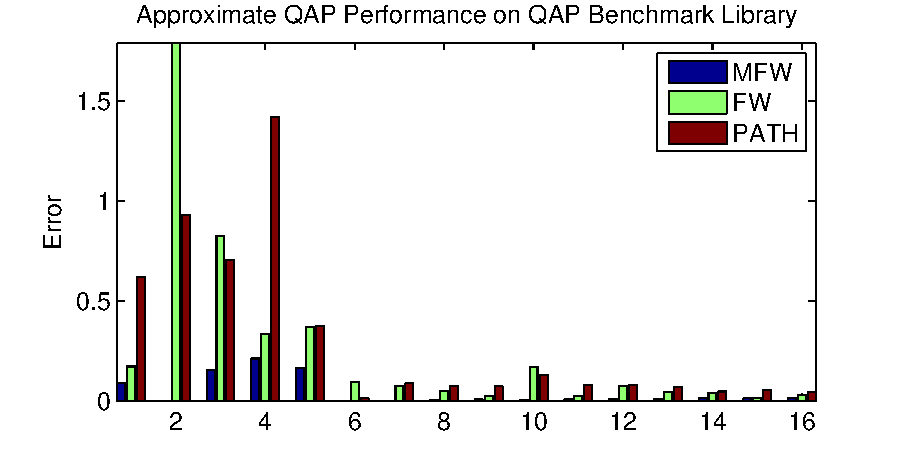
\includegraphics[width=1.0\linewidth]{../figs/benchmarks.pdf}
	\caption{\texttt{QAP}$_3$ outperforms the previous state-of-the-art (PSOA) on all 16 benchmark graph matching problems.  Moreover, \qapa outperforms PSOA on 12 of 16 tests.  For 3 of 16 tests, \qapb achieves the minimum (none of the other algorithms ever find the absolute minimum), as indicated by a black dot.  Let $f_*$ be the minimum and $\mh{f}_x$ be the minimum achieved by algorithm $x$.  Error is $\mh{f}_x/f_*-1$.  }
	\label{fig:fwpath}
\end{figure}





\subsection{LAP vs. QAP} % (fold)
\label{sub:lap_vs_qap}

At surface, LAP and QAP are quite similar.  In fact, the gradient of the LAP objective function is $2AB\T$.

% Much like the QAP objective function from Eq. \eqref{eq:QAP} can be simplified to Eq. \eqref{eq:QAP}, the LAP objective function can be similarly simplified, to give
% \begin{align}
% 	Q_{LAP}= \argmin_{\PmcP} \norm{QA-B}_F^2 = \argmin_{\PmcP} tr(QA B\T).
% \end{align}
% The gradient of the argument on the right-hand-side of the above equation is $2AB\T$.
% Letting $f_{LAP}(Q)=tr(QA B\T)$, the gradient is:
% \begin{align}
% 	% f_{QAP}(Q)	&= -tr(B\T QAQ\T) -tr(QAQ\T B)  &f_{LAP}(Q)&=-tr(AQ\T B\T) \\
% 	% \nabla_{QAP}&= AQB\T+A\T QB               	&
% 	\nabla_{LAP}&=2A B\T.
% \end{align}
% Thus, when $Q=I$, the gradient of the QAP objective function is identical to that of the LAP objective function. Thus, one can use gradient ascent to to solve a LAP.  The gradient of $f'(Q)=\norm{AQ\T-B}_F^2$ is %:
% % \begin{align} \label{eq:grad2}
% 	$\partial f'/\partial Q = 2A B\T$. 
% % \end{align}
Comparing this gradient to the gradient of the QAP objective function---Eq. \eqref{eq:grad}---one can see that when (i) $P^{(j)}$ is the identity matrix and (ii) both $A$ and $B$ are symmetric (for example, for undirected graphs), the two gradients are identical.  Thus, if QAP is initialized at the identity matrix and the graphs are undirected, the first permutation matrix---the output of \emph{Step 2} in our \qap algorithm---is identical to the LAP solution; although the line search will make $P^{(1)}$ not equal the LAP solution in general. %$ \neq Q_{LAP}$, in general.  %Moreoever, projecting a matrix onto the closest permutation matrix can be written as a LAP because of the following relationship:
% \begin{align}
% 	\argmin_{\PmcP} \norm{QA\T - I}_F^2 &= \argmin_{\PmcP} (QA\T-I)\T (QA\T-I) 
% \nonumber\\ &=\argmin_{\PmcP} AQ\T QA\T -2QA\T - II = \argmin_{\PmcP}  -\langle Q, A\T \rangle  
% \end{align}

% In the above simulation, the first iteration of \qap is essentially the only useful one.  Thus, we compare the performance of \texttt{BPI}$\circ$\texttt{LAP} (dark gray).  The performance of LAP and QAP are not statistically different for this simulation.  This suggests that for certain problems, LAP (which is $\mc{O}(n^3)$) is both an efficient and useful approximation to solving $\mc{NP}$-hard graph matching problems. We were unable to find a model for simple graphs in which multiple iterations of \qap improved performance over LAP. %We confirm this intuition by substituting QAP with LAP in the above simulations (black line).  As depicted in the above figures, this intuition is consistent with the numerical results. In other words, while naively one might implement an algorithm with exponential time complexity, LAP, which is only quadratic time complexity, will often suffice.


% subsection lap_vs_qap (end)


\subsection{Algorithm Complexity and leading constants} % (fold)
\label{sub:algorithm_complexity_and_leading_constants}

Both GM and its closely related counterpart, graph isomorphism (GI), are computationally difficult.  There exist no known algorithms for which worst case behavior is polynomial \cite{Fortin1996}.  While GM is known to be $\mc{NP}$-hard, it remains unclear whether GI is in $\mc{P}$, $\mc{NP}$, or its own intermediate complexity class, $\mc{NP}$-isomorphism (or isomorphism-complete).  Yet, for large classes of GI and GM problems, linear or polynomial time algorithms are available \cite{Babai1980}.  Moreover, at worst, it is clear that GI is only ``moderately exponential,'' for example, $\mc{O}(\exp\{n^{1/2 + o(1)}\})$ \cite{Babai1981}.  Unfortunately, even when linear or polynomial time GM or GI algorithms are available for special cases of graphs, the constants are typically unbearably large.  For example, if all graphs have degree less than $k$, there is a linear time algorithm for GI.  However, the hidden constant in this algorithm is $512k^3!$ \cite{Chen1994}.  We therefore determined the average complexity of our algorithm \emph{and} the leading constants.  Figure \ref{fig:scaling} suggests that our algorithm is not just cubic in time, but also has very small leading constants ($\approx 10^{-7}$ seconds), making using this algorithm feasible for even reasonably large graphs.




\begin{figure}[htbp]
	\centering			
	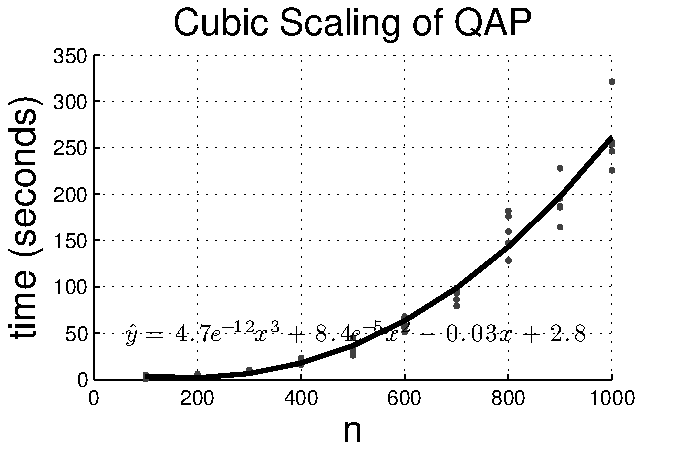
\includegraphics[width=1.0\linewidth]{../figs/digraph_qap2}
	\caption{Performance of \qap as function of number of vertices. Data was sampled from an Erd\"os-R\'enyi model with $p=log(n)/n$.  Each dot represents a single simulation.  The solid line is the best fit cubic function.  Note the leading constant is $10^{-7}$ seconds. }
	\label{fig:scaling}
\end{figure}

% subsection algorithm_complexity_and_leading_constants (end)


\subsection{Brain-Graph Matching} % (fold)
\label{sub:connectome_classification}

A ``connectome'' is a brain-graph in which vertices correspond to (collections of) neurons, and edges correspond to connections between them. The \emph{Caenorhabditis elegans} (\emph{C. elegans}) is a small worm (nematode) with $302$ labeled vertices.  We consider the subgraph with $279$ somatic neurons that form edges with other neurons \cite{WhiteBrenner86, Varshney2011}.  Two distinct kinds of edges exist between vertices: chemical and electrical ``synapses'' (edges). Any pair of vertices may have several edges of each type. Moreover, some of the synapses are hyperedges amongst more than two vertices.    Thus, the connectome of a \emph{C. elegans} may be thought of as a weighted multi-hypergraph, where the weights are the number of edges of each type.  The \qapm algorithm natively operates on weighted or unweighted graphs.  We therefore conducted the following synthetic experiments.  Let $A_{uvz} \in \{0,1,2,\ldots\}$ be the number of synapses from neuron $v$ to neuron $u$ of type $z$ (either chemical or electrical), and let $A_z=\{A_{uv}\}_{u,v \in [279]}$ for $z \in \{e,c\}$ corresponding to the electrical or chemical connectome.  Let $B_{iz}=Q_{iz} A_z Q_{iz}\T$, for some $Q_{iz}$ chosen uniformly at random from $\mc{Q}$ for $i=1,\ldots,s$.  For each $i$ and $z$, obtain $\mh{Q}_{iz}$ using \qapm as described above.  Define ``accuracy'' as $\frac{1}{279}\sum_{uv} Q_{iz} \mh{Q}_{iz}$.  Table \ref{tab:1} shows some summary results of applying \qapm to both $A_c$ and $A_e$ for $s=10$ times.  Note that average solution time is actually smaller than predicted via simulations.  Further note that while the electrical connectome was more difficult, the median number of restarts was less than $30$.  Our stopping criteria on the number of restarts was either (i) perfect assignment or (ii) 30 restarts.  Therefore, this approach achieved perfect assignment sometimes even on this harder assignment problem.

To investigate the performance of \qap using an undirected graph model, we repeated the above analysis using binarized symmeterized versions of the graphs ($A_{uvz}=1$ if and only if $A_{uvz}\geq 1$ or $A_{vuz} \geq 1$).  The resulting summary statistics are nearly identical to those presented in Table \ref{tab:1}, although runtime was less than half the time.

\begin{table}
\caption{Brain-graph matching summary statistics for both the chemical and electrical connectome.  
The table shows the mean (standard deviation) of accuracy, number of restarts, and solution time for both connectomes.  
The maximum number of restarts for both was 30.  The mean number of restarts for the both connectomes is less than 30, implying that our approach found the optimal solution many times, just not always for the electrical connectome.  Both ran very quickly, only requiring tens of seconds.}
	\label{tab:1}
\begin{center}
\begin{tabular}{|l|c|c|c|}
	\hline  	& chemical 	& electrical 	& unit \\ \hline
	Accuracy  		  	& 100  (0)  & 59 (0.30) 	& \% \\
	Restarts 	  		& 3    (0)  & 25 (6.7)  	& \# \\
	Solution Time  		& 42 (0.42)	& 79 (20)  		& sec. \\ \hline
\end{tabular} 
\end{center}
\end{table}

 


\section{Discussion}

This work presents an inexact graph matching algorithm.  Our key insight was to relax the binary constraint to its continuous counterpart---the doubly stochastic matrices---which is the convex hull of the original feasible region.  This insight led to an inexact matching algorithm with a few distinct features. %While others have incorporated the FW algorithm as a subroutine of a graph matching strategy \cite{Zaslavskiy2009}, we modified the FW algorithm for GM in a few ways.  
First, after finding a local solution to the relaxed problem, we project the resulting doubly stochastic matrix onto the set of permutation matrices.  Second, we initialize the algorithm using either the identity matrix or the doubly flat matrix (the matrix where all elements are $1/n$).  These choices seem to us to be the most obvious places to start if one must choose.  Third, if one of those choices does not work, we restart FW with other ``nearby'' initial points.  These modifications facilitate improved performance on \emph{all} the benchmarks we considered.  Moreover, although the algorithm scales cubically with the number of vertices, the leading constants are very small ($\mc{O}(10^{-7})$ seconds), so the algorithm runs quite fast on reasonably sized networks (e.g., $n \approx 100$).  Indeed, on a biologically inspired GM problem, \emph{C. elegans} connectome mapping, this approach was both fast and effective.  

Unfortunately, even with very small leading constants for this algorithm, as $n$ increases, the computational burden gets quite high.  For example, extrapolating the curve of Figure \ref{fig:scaling}, this algorithm would take about 2 years to finish (on a standard laptop from 2011) when $n=20,000$.  We hope to be able to perform GM on graphs much larger than that, given that the number of neurons in even a fly brain, for example, is $\mc{O}(10^5)$.  Therefore, more efficient implementations are of interest.  

Although \qapn consistently found the optimal solution for the \emph{C. elegans} chemical connectome, connectomes for different organisms even within a species are unlikely to be identical. Even if all connectomes of a particular species were identical, measurement error will likely persist \cite{Helmstaedter2011}. Therefore, \texttt{QAP}$_n$'s scientific utility will largely rest on its performance under noisy conditions, which we aim to explore in future work.  

Additional future work might generalize \texttt{QAP}$_n$ in a number of ways.  First, that QAP and LAP are so similar suggests that perhaps one could simply implement a single iteration of QAP starting from the identity.  While not changing the order of complexity, it could reduce computational time by at least an order of magnitude, without drastically changing performance properties (because convergence typically requires around $5-15$ iterations for the graphs we tested).  The relative performance/computational cost trade-off merits further theoretical investigations.  Second, the most ``costly'' subroutine is LAP.  Fortunately, LAP is a quadratic optimization problem with linear constraints.  A number of parallelized optimization strategies could therefore potentially be brought to bear on this problem \cite{Boyd2011}.  Third, our matrices have certain special properties, namely sparsity, which makes more efficient algorithms (such as ``active set'' algorithms) readily available for further speed increases.  Fourth, for brain-graphs, we have some prior information that could easily be incorporated in the form of vertex attributes.  For example, position in the brain, cell type, etc., could be used to measure ``dissimilarity'' between vertices.  The objective function could then be modified to give
\begin{align} \label{eq:Jqap}
	\mt{Q}_{AB}= \argmin_{Q \in \mc{D}} \norm{Q A Q\T - B}^2_F + \lambda J(Q),
\end{align}
where $J(Q)$ is a dissimilarity based penalty and $\lambda$ is a hyper-parameter.  Finally, although this approach natively operates on both unweighted and weighted graphs, multi-graphs are a possible extension.

In conclusion, this manuscript has presented a GM algorithm that is fast, effective, and easily generalizable.  To facilitate further development and applications, all the code and data used in this manuscript is available from the first author's website, \url{http://jovo.me}.












% use section* for acknowledgement
\ifCLASSOPTIONcompsoc
  % The Computer Society usually uses the plural form
  \section*{Acknowledgments}
\else
  % regular IEEE prefers the singular form
  \section*{Acknowledgment}
\fi

% This work was partially supported by the Research Program in Applied Neuroscience. 

% Can use something like this to put references on a page
% by themselves when using endfloat and the captionsoff option.
\ifCLASSOPTIONcaptionsoff
  \newpage
\fi

\bibliography{/Users/jovo/Research/latex/library}
\bibliographystyle{IEEEtran}

\begin{IEEEbiographynophoto}{Joshua T. Vogelstein}
% Joshua T. Vogelstein is a spritely young man, engulfed in a novel post-buddhist metaphor.

\end{IEEEbiographynophoto}


% insert where needed to balance the two columns on the last page with
% biographies
%\newpage

\begin{IEEEbiographynophoto}{John C.~Conroy}
% John C.~Conroy seems to basically always be right. He also publishes sometimes.

\end{IEEEbiographynophoto}

\begin{IEEEbiographynophoto}{Lou Podrazik}

\end{IEEEbiographynophoto}

\begin{IEEEbiographynophoto}{Steve Kratzer}

\end{IEEEbiographynophoto}



\begin{IEEEbiographynophoto}{R. Jacob Vogelstein}
% R. Jacob Vogelstein received the Sc.B. degree in neuroengineering from Brown University, Providence, RI, and the Ph.D. degree in biomedical engineering from the Johns Hopkins University School of Medicine, Baltimore, MD.  He currently oversees the Applied Neuroscience programs at the Johns Hopkins University (JHU) Applied Physics Laboratory as an Assistant Program Manager, and has an appointment as an Assistant Research Professor at the JHU Whiting School of Engineering’s Department of Electrical and Computer Engineering. He has worked on neuroscience technology for over a decade, focusing primarily on neuromorphic systems and closed-loop brain–machine interfaces. His research has been featured in a number of prominent scientific and engineering journals including the IEEE Transactions on Neural Systems and Rehabilitation Engineering, the IEEE Transactions on Biomedical Circuits and Systems, and the IEEE Transactions on Neural Networks.  
\end{IEEEbiographynophoto}

\begin{IEEEbiographynophoto}{Carey E. Priebe}
% Buddha in training.
\end{IEEEbiographynophoto}

% Can be used to pull up biographies so that the bottom of the last one
% is flush with the other column.
% \enlargethispage{-5in}

\end{document}



